\section{Versuchsaufbau und Durchführung}
\label{sec:Durchführung}

\subsection{Versuchsaufbau}
\label{subsec:Versuchsaufbau}
Der Versuchsaufbau besteht aus einer Kammer mit einem Plattenkondensator, der eine kleine Öffnung an der Oberseite aufweist. 
Diese Oberseite wird zum Einspritzen von zerstäubten Öltröpfchen verwendet. Die Platten des Kondensators haben einen Abstand 
von $d = (7,6250 \pm 0,0051) \, \si{\milli\meter}$.

Um die Tröpfchen gut sichtbar zu machen, werden sie seitlich von einer Halogenlampe beleuchtet. Die Temperatur der Luft in der 
Kammer wird mit einem Thermowiderstand kontrolliert, dessen Wert an einem Multimeter abgelesen werden kann. Ebenso kann die 
Spannung zwischen den beiden Kondensatorplatten an einem Multimeter abgelesen werden.

Durch das Zerstäuben sind die meisten Öltröpfchen geladen, während einige nicht geladen sind. Die nicht geladenen Tröpfchen 
können durch ein schwach radioaktives $\alpha$-Präparat ionisiert werden. Durch einen Schalter kann das Präparat abgeschirmt 
oder aktiviert werden.

Die Polung der Kondensatorplatten kann mit einem Schalter geändert werden. Mit einer Libelle kann überprüft und eingestellt 
werden, ob die Apparatur gerade steht. Die Tröpfchen können mit einem Mikroskop beobachtet werden.

Der Versuchsaufbau ist in Abbildung \ref{fig:Versuchsaufbau} dargestellt.

\begin{figure}[H]
    \centering
    \caption{Schematischer Aufbau der Versuchsappartatur zum Millikan-Öltröpchen-Versuch.\cite{1}}
    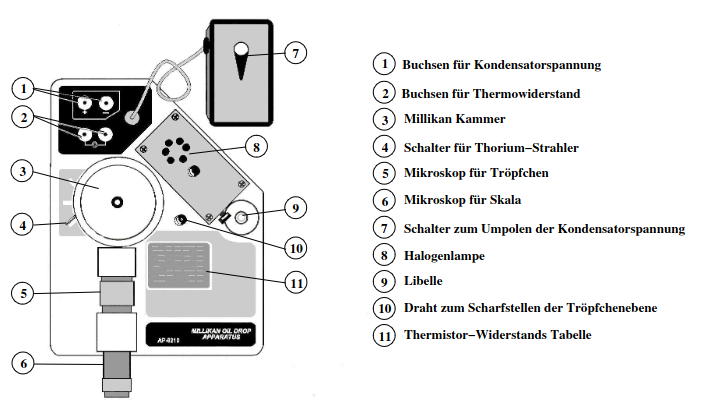
\includegraphics[width=\textwidth]{Bilder/Versuchsaufbau.png}
    \label{fig:Versuchsaufbau}
\end{figure}


\subsection{Durchführung}
\label{subsec:Durchführung}

Zu Beginn wird die Ausrichtung der Apparatur überprüft, um sicherzustellen, dass sie waagerecht steht. Dies wird mithilfe einer 
Libelle durchgeführt.Außerdem wird durch fokussieren auf eine Nadelspitze die Linse eingestellt.
Anschließend werden die Kondensatorplatten geerdet und Öltröpfchen in die Kammer eingesprüht. Während des 
Einsprühens wird mithilfe eines Mikroskops überwacht, wie viele Tröpfchen in die Kammer gelangen.

Nun werden bei zwei verschiedenen Spannungen 22 verschiedene Tröpfchen beobachtet. Dabei werden die Zeiten für den Aufstieg 
und den Abstieg eines Tröpfchens über eine festgelegte Strecke jeweils drei Mal gemessen. Vor jeder Messung wird der Wert 
der Temperatur für jedes Tröpfchen erfasst.

Die verwendeten Spannungen betragen 200 V und 230 V. Durch das Umpolen mithilfe des Schalters werden die Tröpfchen entweder 
in Aufwärts- oder Abwärtsbewegung gebracht.


